% Options for packages loaded elsewhere
\PassOptionsToPackage{unicode}{hyperref}
\PassOptionsToPackage{hyphens}{url}
\PassOptionsToPackage{dvipsnames,svgnames,x11names}{xcolor}
%
\documentclass[
  letterpaper,
  DIV=11,
  numbers=noendperiod]{scrartcl}

\usepackage{amsmath,amssymb}
\usepackage{iftex}
\ifPDFTeX
  \usepackage[T1]{fontenc}
  \usepackage[utf8]{inputenc}
  \usepackage{textcomp} % provide euro and other symbols
\else % if luatex or xetex
  \usepackage{unicode-math}
  \defaultfontfeatures{Scale=MatchLowercase}
  \defaultfontfeatures[\rmfamily]{Ligatures=TeX,Scale=1}
\fi
\usepackage{lmodern}
\ifPDFTeX\else  
    % xetex/luatex font selection
\fi
% Use upquote if available, for straight quotes in verbatim environments
\IfFileExists{upquote.sty}{\usepackage{upquote}}{}
\IfFileExists{microtype.sty}{% use microtype if available
  \usepackage[]{microtype}
  \UseMicrotypeSet[protrusion]{basicmath} % disable protrusion for tt fonts
}{}
\makeatletter
\@ifundefined{KOMAClassName}{% if non-KOMA class
  \IfFileExists{parskip.sty}{%
    \usepackage{parskip}
  }{% else
    \setlength{\parindent}{0pt}
    \setlength{\parskip}{6pt plus 2pt minus 1pt}}
}{% if KOMA class
  \KOMAoptions{parskip=half}}
\makeatother
\usepackage{xcolor}
\setlength{\emergencystretch}{3em} % prevent overfull lines
\setcounter{secnumdepth}{-\maxdimen} % remove section numbering
% Make \paragraph and \subparagraph free-standing
\makeatletter
\ifx\paragraph\undefined\else
  \let\oldparagraph\paragraph
  \renewcommand{\paragraph}{
    \@ifstar
      \xxxParagraphStar
      \xxxParagraphNoStar
  }
  \newcommand{\xxxParagraphStar}[1]{\oldparagraph*{#1}\mbox{}}
  \newcommand{\xxxParagraphNoStar}[1]{\oldparagraph{#1}\mbox{}}
\fi
\ifx\subparagraph\undefined\else
  \let\oldsubparagraph\subparagraph
  \renewcommand{\subparagraph}{
    \@ifstar
      \xxxSubParagraphStar
      \xxxSubParagraphNoStar
  }
  \newcommand{\xxxSubParagraphStar}[1]{\oldsubparagraph*{#1}\mbox{}}
  \newcommand{\xxxSubParagraphNoStar}[1]{\oldsubparagraph{#1}\mbox{}}
\fi
\makeatother

\usepackage{color}
\usepackage{fancyvrb}
\newcommand{\VerbBar}{|}
\newcommand{\VERB}{\Verb[commandchars=\\\{\}]}
\DefineVerbatimEnvironment{Highlighting}{Verbatim}{commandchars=\\\{\}}
% Add ',fontsize=\small' for more characters per line
\usepackage{framed}
\definecolor{shadecolor}{RGB}{241,243,245}
\newenvironment{Shaded}{\begin{snugshade}}{\end{snugshade}}
\newcommand{\AlertTok}[1]{\textcolor[rgb]{0.68,0.00,0.00}{#1}}
\newcommand{\AnnotationTok}[1]{\textcolor[rgb]{0.37,0.37,0.37}{#1}}
\newcommand{\AttributeTok}[1]{\textcolor[rgb]{0.40,0.45,0.13}{#1}}
\newcommand{\BaseNTok}[1]{\textcolor[rgb]{0.68,0.00,0.00}{#1}}
\newcommand{\BuiltInTok}[1]{\textcolor[rgb]{0.00,0.23,0.31}{#1}}
\newcommand{\CharTok}[1]{\textcolor[rgb]{0.13,0.47,0.30}{#1}}
\newcommand{\CommentTok}[1]{\textcolor[rgb]{0.37,0.37,0.37}{#1}}
\newcommand{\CommentVarTok}[1]{\textcolor[rgb]{0.37,0.37,0.37}{\textit{#1}}}
\newcommand{\ConstantTok}[1]{\textcolor[rgb]{0.56,0.35,0.01}{#1}}
\newcommand{\ControlFlowTok}[1]{\textcolor[rgb]{0.00,0.23,0.31}{\textbf{#1}}}
\newcommand{\DataTypeTok}[1]{\textcolor[rgb]{0.68,0.00,0.00}{#1}}
\newcommand{\DecValTok}[1]{\textcolor[rgb]{0.68,0.00,0.00}{#1}}
\newcommand{\DocumentationTok}[1]{\textcolor[rgb]{0.37,0.37,0.37}{\textit{#1}}}
\newcommand{\ErrorTok}[1]{\textcolor[rgb]{0.68,0.00,0.00}{#1}}
\newcommand{\ExtensionTok}[1]{\textcolor[rgb]{0.00,0.23,0.31}{#1}}
\newcommand{\FloatTok}[1]{\textcolor[rgb]{0.68,0.00,0.00}{#1}}
\newcommand{\FunctionTok}[1]{\textcolor[rgb]{0.28,0.35,0.67}{#1}}
\newcommand{\ImportTok}[1]{\textcolor[rgb]{0.00,0.46,0.62}{#1}}
\newcommand{\InformationTok}[1]{\textcolor[rgb]{0.37,0.37,0.37}{#1}}
\newcommand{\KeywordTok}[1]{\textcolor[rgb]{0.00,0.23,0.31}{\textbf{#1}}}
\newcommand{\NormalTok}[1]{\textcolor[rgb]{0.00,0.23,0.31}{#1}}
\newcommand{\OperatorTok}[1]{\textcolor[rgb]{0.37,0.37,0.37}{#1}}
\newcommand{\OtherTok}[1]{\textcolor[rgb]{0.00,0.23,0.31}{#1}}
\newcommand{\PreprocessorTok}[1]{\textcolor[rgb]{0.68,0.00,0.00}{#1}}
\newcommand{\RegionMarkerTok}[1]{\textcolor[rgb]{0.00,0.23,0.31}{#1}}
\newcommand{\SpecialCharTok}[1]{\textcolor[rgb]{0.37,0.37,0.37}{#1}}
\newcommand{\SpecialStringTok}[1]{\textcolor[rgb]{0.13,0.47,0.30}{#1}}
\newcommand{\StringTok}[1]{\textcolor[rgb]{0.13,0.47,0.30}{#1}}
\newcommand{\VariableTok}[1]{\textcolor[rgb]{0.07,0.07,0.07}{#1}}
\newcommand{\VerbatimStringTok}[1]{\textcolor[rgb]{0.13,0.47,0.30}{#1}}
\newcommand{\WarningTok}[1]{\textcolor[rgb]{0.37,0.37,0.37}{\textit{#1}}}

\providecommand{\tightlist}{%
  \setlength{\itemsep}{0pt}\setlength{\parskip}{0pt}}\usepackage{longtable,booktabs,array}
\usepackage{calc} % for calculating minipage widths
% Correct order of tables after \paragraph or \subparagraph
\usepackage{etoolbox}
\makeatletter
\patchcmd\longtable{\par}{\if@noskipsec\mbox{}\fi\par}{}{}
\makeatother
% Allow footnotes in longtable head/foot
\IfFileExists{footnotehyper.sty}{\usepackage{footnotehyper}}{\usepackage{footnote}}
\makesavenoteenv{longtable}
\usepackage{graphicx}
\makeatletter
\newsavebox\pandoc@box
\newcommand*\pandocbounded[1]{% scales image to fit in text height/width
  \sbox\pandoc@box{#1}%
  \Gscale@div\@tempa{\textheight}{\dimexpr\ht\pandoc@box+\dp\pandoc@box\relax}%
  \Gscale@div\@tempb{\linewidth}{\wd\pandoc@box}%
  \ifdim\@tempb\p@<\@tempa\p@\let\@tempa\@tempb\fi% select the smaller of both
  \ifdim\@tempa\p@<\p@\scalebox{\@tempa}{\usebox\pandoc@box}%
  \else\usebox{\pandoc@box}%
  \fi%
}
% Set default figure placement to htbp
\def\fps@figure{htbp}
\makeatother

\KOMAoption{captions}{tableheading}
\makeatletter
\@ifpackageloaded{caption}{}{\usepackage{caption}}
\AtBeginDocument{%
\ifdefined\contentsname
  \renewcommand*\contentsname{Table of contents}
\else
  \newcommand\contentsname{Table of contents}
\fi
\ifdefined\listfigurename
  \renewcommand*\listfigurename{List of Figures}
\else
  \newcommand\listfigurename{List of Figures}
\fi
\ifdefined\listtablename
  \renewcommand*\listtablename{List of Tables}
\else
  \newcommand\listtablename{List of Tables}
\fi
\ifdefined\figurename
  \renewcommand*\figurename{Figure}
\else
  \newcommand\figurename{Figure}
\fi
\ifdefined\tablename
  \renewcommand*\tablename{Table}
\else
  \newcommand\tablename{Table}
\fi
}
\@ifpackageloaded{float}{}{\usepackage{float}}
\floatstyle{ruled}
\@ifundefined{c@chapter}{\newfloat{codelisting}{h}{lop}}{\newfloat{codelisting}{h}{lop}[chapter]}
\floatname{codelisting}{Listing}
\newcommand*\listoflistings{\listof{codelisting}{List of Listings}}
\makeatother
\makeatletter
\makeatother
\makeatletter
\@ifpackageloaded{caption}{}{\usepackage{caption}}
\@ifpackageloaded{subcaption}{}{\usepackage{subcaption}}
\makeatother

\usepackage{bookmark}

\IfFileExists{xurl.sty}{\usepackage{xurl}}{} % add URL line breaks if available
\urlstyle{same} % disable monospaced font for URLs
\hypersetup{
  pdftitle={HW2},
  colorlinks=true,
  linkcolor={blue},
  filecolor={Maroon},
  citecolor={Blue},
  urlcolor={Blue},
  pdfcreator={LaTeX via pandoc}}


\title{HW2}
\author{}
\date{}

\begin{document}
\maketitle


\begin{Shaded}
\begin{Highlighting}[]
\FunctionTok{library}\NormalTok{(sf)}
\end{Highlighting}
\end{Shaded}

\begin{verbatim}
Linking to GEOS 3.13.1, GDAL 3.4.3, PROJ 8.2.0; sf_use_s2() is TRUE
\end{verbatim}

\begin{Shaded}
\begin{Highlighting}[]
\FunctionTok{library}\NormalTok{(terra)}
\end{Highlighting}
\end{Shaded}

\begin{verbatim}
terra 1.8.54
\end{verbatim}

\begin{Shaded}
\begin{Highlighting}[]
\FunctionTok{library}\NormalTok{(ggplot2) }
\FunctionTok{library}\NormalTok{(raster)}
\end{Highlighting}
\end{Shaded}

\begin{verbatim}
Loading required package: sp
\end{verbatim}

\begin{verbatim}
The legacy packages maptools, rgdal, and rgeos, underpinning the sp package,
which was just loaded, will retire in October 2023.
Please refer to R-spatial evolution reports for details, especially
https://r-spatial.org/r/2023/05/15/evolution4.html.
It may be desirable to make the sf package available;
package maintainers should consider adding sf to Suggests:.
The sp package is now running under evolution status 2
     (status 2 uses the sf package in place of rgdal)
\end{verbatim}

\begin{Shaded}
\begin{Highlighting}[]
\CommentTok{\#load DEM raster }
\NormalTok{dem0 }\OtherTok{\textless{}{-}} \FunctionTok{rast}\NormalTok{(}\StringTok{"/carl{-}data/shared/users/sanshre/DPON\_2024/Stillwater/ODM\_DSM/2024\_01\_03\_ST\_M\_odm\_dsm\_modified.tif"}\NormalTok{)}
\NormalTok{dem1 }\OtherTok{\textless{}{-}} \FunctionTok{rast}\NormalTok{(}\StringTok{"/carl{-}data/shared/users/sanshre/DPON\_2024/Stillwater/ODM\_DSM/2024\_04\_29\_ST\_M\_odm\_dsm.tif"}\NormalTok{)}
\NormalTok{dem0\_resampled }\OtherTok{\textless{}{-}} \FunctionTok{resample}\NormalTok{(dem0, dem1)}
\NormalTok{DEM }\OtherTok{\textless{}{-}}\NormalTok{ dem1 }\SpecialCharTok{{-}}\NormalTok{ dem0\_resampled}

\NormalTok{shapfil }\OtherTok{\textless{}{-}} \FunctionTok{st\_read}\NormalTok{(}\StringTok{"/carl{-}data/shared/carl/gcp\_detail/shapefile\_2024\_stw/shape\_grid\_ST\_02\_20\_2024.shp"}\NormalTok{)}
\end{Highlighting}
\end{Shaded}

\begin{verbatim}
Reading layer `shape_grid_ST_02_20_2024' from data source 
  `/carl-data/shared/carl/gcp_detail/shapefile_2024_stw/shape_grid_ST_02_20_2024.shp' 
  using driver `ESRI Shapefile'
Simple feature collection with 2418 features and 1 field
Geometry type: POLYGON
Dimension:     XY
Bounding box:  xmin: 671661.4 ymin: 3999098 xmax: 671743.3 ymax: 3999271
Projected CRS: WGS 84 / UTM zone 14N
\end{verbatim}

\begin{Shaded}
\begin{Highlighting}[]
\NormalTok{shapfil }\OtherTok{\textless{}{-}} \FunctionTok{st\_transform}\NormalTok{(shapfil, }\AttributeTok{crs =} \FunctionTok{crs}\NormalTok{(DEM, }\AttributeTok{proj =} \ConstantTok{TRUE}\NormalTok{))}
\end{Highlighting}
\end{Shaded}

\begin{Shaded}
\begin{Highlighting}[]
\CommentTok{\#load orthophoto and calculate ndvi}
\NormalTok{orthophoto }\OtherTok{\textless{}{-}} \FunctionTok{rast}\NormalTok{(}\StringTok{"/carl{-}data/shared/users/sanshre/DPON\_2024/Stillwater/DPON{-}2024{-}04{-}29/M\_combined\_newV/odm\_orthophoto/odm\_orthophoto.tif"}\NormalTok{)}
\NormalTok{nir }\OtherTok{\textless{}{-}}\NormalTok{ orthophoto[[}\DecValTok{4}\NormalTok{]]}
\NormalTok{red }\OtherTok{\textless{}{-}}\NormalTok{ orthophoto[[}\DecValTok{1}\NormalTok{]]}
\NormalTok{ndvi }\OtherTok{\textless{}{-}}\NormalTok{ (nir}\SpecialCharTok{{-}}\NormalTok{red) }\SpecialCharTok{/}\NormalTok{ (nir}\SpecialCharTok{+}\NormalTok{red}\FloatTok{+0.000001}\NormalTok{)}
\end{Highlighting}
\end{Shaded}

\begin{Shaded}
\begin{Highlighting}[]
\CommentTok{\# Create empty list to store results}
\NormalTok{results }\OtherTok{\textless{}{-}} \FunctionTok{list}\NormalTok{()}

\CommentTok{\# Loop through each FID}
\ControlFlowTok{for}\NormalTok{ (fid }\ControlFlowTok{in}\NormalTok{ shapfil}\SpecialCharTok{$}\NormalTok{FID) \{}
  
  \CommentTok{\# Get the polygon geometry for the current FID}
\NormalTok{  plot\_geom }\OtherTok{\textless{}{-}}\NormalTok{ shapfil[shapfil}\SpecialCharTok{$}\NormalTok{FID }\SpecialCharTok{==}\NormalTok{ fid, ]}
  
  \CommentTok{\# Crop/mask NDVI to the plot}
\NormalTok{  vi\_plot }\OtherTok{\textless{}{-}} \FunctionTok{crop}\NormalTok{(ndvi, plot\_geom)}
\NormalTok{  vi\_plot }\OtherTok{\textless{}{-}} \FunctionTok{mask}\NormalTok{(vi\_plot, plot\_geom)}
  
  \CommentTok{\# Crop/mask and resample height to the same plot}
\NormalTok{  ht\_plot }\OtherTok{\textless{}{-}} \FunctionTok{crop}\NormalTok{(DEM, plot\_geom)}
\NormalTok{  ht\_plot }\OtherTok{\textless{}{-}} \FunctionTok{mask}\NormalTok{(ht\_plot, plot\_geom)}
\NormalTok{  ht\_plot }\OtherTok{\textless{}{-}} \FunctionTok{resample}\NormalTok{(ht\_plot, vi\_plot) }
                      
  \CommentTok{\# Calculate average plot plant height }
\NormalTok{  avg\_height }\OtherTok{\textless{}{-}} \FunctionTok{mean}\NormalTok{(}\FunctionTok{values}\NormalTok{(ht\_plot), }\AttributeTok{na.rm =} \ConstantTok{TRUE}\NormalTok{) }
  
  \CommentTok{\# Calculate the lower and upper threshold }
\NormalTok{  lower\_threshold }\OtherTok{\textless{}{-}}\NormalTok{ avg\_height }\SpecialCharTok{*} \FloatTok{0.80}
\NormalTok{  upper\_threshold }\OtherTok{\textless{}{-}}\NormalTok{ avg\_height }\SpecialCharTok{*} \FloatTok{0.90} 
  
  \CommentTok{\# Create mask for pixels within that height thresholds}
\NormalTok{  height\_mask }\OtherTok{\textless{}{-}}\NormalTok{ ht\_plot }\SpecialCharTok{\textgreater{}=}\NormalTok{ lower\_threshold }\SpecialCharTok{\&}\NormalTok{ ht\_plot }\SpecialCharTok{\textless{}=}\NormalTok{ upper\_threshold }
  
  \CommentTok{\# Apply mask to VI plot}
\NormalTok{  vi\_sub }\OtherTok{\textless{}{-}} \FunctionTok{mask}\NormalTok{(vi\_plot, height\_mask, }\AttributeTok{maskvalue =} \DecValTok{0}\NormalTok{)}
  
  \CommentTok{\# Extract VI as numeric }
\NormalTok{  vi\_values }\OtherTok{\textless{}{-}} \FunctionTok{na.omit}\NormalTok{(}\FunctionTok{values}\NormalTok{(vi\_sub))}
  
  \CommentTok{\# Compute plot{-}level statistics}
\NormalTok{  vi\_stats }\OtherTok{\textless{}{-}} \FunctionTok{list}\NormalTok{(}
    \AttributeTok{FID =}\NormalTok{ fid,}
    \AttributeTok{mean =} \FunctionTok{mean}\NormalTok{(vi\_values, }\AttributeTok{na.rm =} \ConstantTok{TRUE}\NormalTok{),}
    \AttributeTok{sd =} \FunctionTok{sd}\NormalTok{(vi\_values, }\AttributeTok{na.rm =} \ConstantTok{TRUE}\NormalTok{),}
    \AttributeTok{skewness =}\NormalTok{ e1071}\SpecialCharTok{::}\FunctionTok{skewness}\NormalTok{(vi\_values, }\AttributeTok{na.rm =} \ConstantTok{TRUE}\NormalTok{),}
    \AttributeTok{kurtosis =}\NormalTok{ e1071}\SpecialCharTok{::}\FunctionTok{kurtosis}\NormalTok{(vi\_values, }\AttributeTok{na.rm =} \ConstantTok{TRUE}\NormalTok{)}
\NormalTok{  )}

  \CommentTok{\# Store results}
\NormalTok{  results[[}\FunctionTok{as.character}\NormalTok{(fid)]] }\OtherTok{\textless{}{-}}\NormalTok{ vi\_stats}
\NormalTok{\}}
\NormalTok{viresults\_df }\OtherTok{\textless{}{-}} \FunctionTok{do.call}\NormalTok{(rbind, }\FunctionTok{lapply}\NormalTok{(results, as.data.frame))}
\NormalTok{results\_df }\OtherTok{\textless{}{-}} \FunctionTok{data.frame}\NormalTok{(}\AttributeTok{FID =} \FunctionTok{names}\NormalTok{(results), viresults\_df)}
\FunctionTok{write.csv}\NormalTok{(results\_df, }\StringTok{"ndvi\_stats\_by\_plot.csv"}\NormalTok{, }\AttributeTok{row.names =} \ConstantTok{FALSE}\NormalTok{)}
\end{Highlighting}
\end{Shaded}

\begin{Shaded}
\begin{Highlighting}[]
\CommentTok{\# Load necessary data}
\FunctionTok{library}\NormalTok{(dplyr)}
\end{Highlighting}
\end{Shaded}

\begin{verbatim}

Attaching package: 'dplyr'
\end{verbatim}

\begin{verbatim}
The following objects are masked from 'package:raster':

    intersect, select, union
\end{verbatim}

\begin{verbatim}
The following objects are masked from 'package:terra':

    intersect, union
\end{verbatim}

\begin{verbatim}
The following objects are masked from 'package:stats':

    filter, lag
\end{verbatim}

\begin{verbatim}
The following objects are masked from 'package:base':

    intersect, setdiff, setequal, union
\end{verbatim}

\begin{Shaded}
\begin{Highlighting}[]
\NormalTok{results\_df }\OtherTok{\textless{}{-}} \FunctionTok{read.csv}\NormalTok{(}\StringTok{"ndvi\_stats\_by\_plot.csv"}\NormalTok{) }\SpecialCharTok{\%\textgreater{}\%} 
  \FunctionTok{as\_tibble}\NormalTok{()}
\NormalTok{byd\_rating }\OtherTok{\textless{}{-}} \FunctionTok{read.csv}\NormalTok{(}\StringTok{"/carl{-}data/home/arpoude/Desktop/gabor/FIDwithRating.csv"}\NormalTok{) }\SpecialCharTok{\%\textgreater{}\%} 
  \FunctionTok{as\_tibble}\NormalTok{()}
\NormalTok{byd\_rating}
\end{Highlighting}
\end{Shaded}

\begin{verbatim}
# A tibble: 1,951 x 11
       X nursery_id plot_id     x     y   FID    lr   byd yield_st sgc_la
   <int>      <int>   <int> <int> <int> <int> <int> <int>    <dbl>  <int>
 1     1         60       1     2     1     1     3     5     32.6      4
 2     2         60      10    11     1    10    NA     2     29.7      1
 3     3         60     100     2    10   559     2     1     33.8      3
 4     4         60     101     2    11   621     3     3     20.8      3
 5     5         60     102     3    11   622     2     2     21.5      1
 6     6         60     103     4    11   623     2     4     29.9      0
 7     7         60     104     5    11   624     1     1     34.3      1
 8     8         60     105     6    11   625     2     2     40.9      1
 9     9         60     106     7    11   626     2     1     36.3      2
10    10         60     107     8    11   627     4     1     44.1      3
# i 1,941 more rows
# i 1 more variable: yield_la <dbl>
\end{verbatim}

\begin{Shaded}
\begin{Highlighting}[]
\CommentTok{\# Merge datasets by FID}
\NormalTok{full\_data }\OtherTok{\textless{}{-}} \FunctionTok{right\_join}\NormalTok{(results\_df, byd\_rating, }\AttributeTok{by =} \StringTok{"FID"}\NormalTok{)}
\end{Highlighting}
\end{Shaded}

\begin{Shaded}
\begin{Highlighting}[]
\CommentTok{\#make features }
\NormalTok{full\_data }\OtherTok{\textless{}{-}}\NormalTok{ full\_data }\SpecialCharTok{\%\textgreater{}\%}
  \FunctionTok{mutate}\NormalTok{(}
    \AttributeTok{mean\_only =}\NormalTok{ mean,}
    \AttributeTok{mean\_sd =}\NormalTok{ mean }\SpecialCharTok{*}\NormalTok{ sd,}
    \AttributeTok{mean\_sd\_skew =}\NormalTok{ mean }\SpecialCharTok{*}\NormalTok{ sd }\SpecialCharTok{*}\NormalTok{ skewness,}
    \AttributeTok{mean\_sd\_skew\_kurt =}\NormalTok{ mean }\SpecialCharTok{*}\NormalTok{ sd }\SpecialCharTok{*}\NormalTok{ skewness }\SpecialCharTok{*}\NormalTok{ kurtosis}
\NormalTok{  )}

\CommentTok{\# Select only numeric features for PCA}
\NormalTok{features\_df }\OtherTok{\textless{}{-}}\NormalTok{ full\_data }\SpecialCharTok{\%\textgreater{}\%}
  \FunctionTok{select}\NormalTok{(mean\_only, mean\_sd, mean\_sd\_skew, mean\_sd\_skew\_kurt)}
\NormalTok{features\_df\_clean }\OtherTok{\textless{}{-}} \FunctionTok{na.omit}\NormalTok{(features\_df)}

\CommentTok{\# Perform PCA}
\NormalTok{pca\_res }\OtherTok{\textless{}{-}} \FunctionTok{prcomp}\NormalTok{(features\_df\_clean, }\AttributeTok{center =} \ConstantTok{TRUE}\NormalTok{, }\AttributeTok{scale. =} \ConstantTok{TRUE}\NormalTok{)}

\NormalTok{full\_data\_clean }\OtherTok{\textless{}{-}}\NormalTok{ full\_data[}\FunctionTok{complete.cases}\NormalTok{(features\_df),]}

\CommentTok{\# Extract PCA scores and add FID + BYD rating}
\NormalTok{pca\_scores\_df }\OtherTok{\textless{}{-}} \FunctionTok{as.data.frame}\NormalTok{(pca\_res}\SpecialCharTok{$}\NormalTok{x) }\SpecialCharTok{\%\textgreater{}\%}
  \FunctionTok{mutate}\NormalTok{(}\AttributeTok{FID =}\NormalTok{ full\_data\_clean}\SpecialCharTok{$}\NormalTok{FID,}
         \AttributeTok{BYD\_rating =}\NormalTok{ full\_data\_clean}\SpecialCharTok{$}\NormalTok{byd)}
\NormalTok{pca\_scores\_df\_clean }\OtherTok{\textless{}{-}}\NormalTok{ pca\_scores\_df }\SpecialCharTok{\%\textgreater{}\%} 
  \FunctionTok{filter}\NormalTok{(}\SpecialCharTok{!}\FunctionTok{is.na}\NormalTok{(BYD\_rating))}
\end{Highlighting}
\end{Shaded}

\begin{Shaded}
\begin{Highlighting}[]
\FunctionTok{library}\NormalTok{(caret)}
\end{Highlighting}
\end{Shaded}

\begin{verbatim}
Loading required package: lattice
\end{verbatim}

\begin{Shaded}
\begin{Highlighting}[]
\FunctionTok{set.seed}\NormalTok{(}\DecValTok{123}\NormalTok{)  }\CommentTok{\# for reproducibility}

\CommentTok{\# Create a training (70\%) and temp (30\%) split}
\NormalTok{train\_index }\OtherTok{\textless{}{-}} \FunctionTok{createDataPartition}\NormalTok{(pca\_scores\_df\_clean}\SpecialCharTok{$}\NormalTok{BYD\_rating, }\AttributeTok{p =} \FloatTok{0.7}\NormalTok{, }\AttributeTok{list =} \ConstantTok{FALSE}\NormalTok{)}
\NormalTok{train\_data }\OtherTok{\textless{}{-}}\NormalTok{ pca\_scores\_df[train\_index, ]}
\NormalTok{temp\_data  }\OtherTok{\textless{}{-}}\NormalTok{ pca\_scores\_df[}\SpecialCharTok{{-}}\NormalTok{train\_index, ]}

\CommentTok{\# Split temp\_data into validation (15\%) and testing (15\%)}
\NormalTok{val\_index }\OtherTok{\textless{}{-}} \FunctionTok{createDataPartition}\NormalTok{(temp\_data}\SpecialCharTok{$}\NormalTok{BYD\_rating, }\AttributeTok{p =} \FloatTok{0.5}\NormalTok{, }\AttributeTok{list =} \ConstantTok{FALSE}\NormalTok{)}
\NormalTok{val\_data }\OtherTok{\textless{}{-}}\NormalTok{ temp\_data[val\_index, ]}
\NormalTok{test\_data }\OtherTok{\textless{}{-}}\NormalTok{ temp\_data[}\SpecialCharTok{{-}}\NormalTok{val\_index, ]}

\CommentTok{\#Using all PCs}
\NormalTok{pc\_cols }\OtherTok{\textless{}{-}} \FunctionTok{grep}\NormalTok{(}\StringTok{"\^{}PC"}\NormalTok{, }\FunctionTok{names}\NormalTok{(train\_data), }\AttributeTok{value =} \ConstantTok{TRUE}\NormalTok{)}
\NormalTok{formula }\OtherTok{\textless{}{-}} \FunctionTok{as.formula}\NormalTok{(}\FunctionTok{paste}\NormalTok{(}\StringTok{"BYD\_rating \textasciitilde{}"}\NormalTok{, }\FunctionTok{paste}\NormalTok{(pc\_cols, }\AttributeTok{collapse =} \StringTok{" + "}\NormalTok{)))}

\CommentTok{\# Fit model on training set}
\NormalTok{lm\_model }\OtherTok{\textless{}{-}} \FunctionTok{lm}\NormalTok{(formula, }\AttributeTok{data =}\NormalTok{ train\_data)}

\CommentTok{\# View summary}
\FunctionTok{summary}\NormalTok{(lm\_model)}
\end{Highlighting}
\end{Shaded}

\begin{verbatim}

Call:
lm(formula = formula, data = train_data)

Residuals:
    Min      1Q  Median      3Q     Max 
-2.4604 -0.7651 -0.1190  0.6997  3.6510 

Coefficients:
            Estimate Std. Error t value Pr(>|t|)    
(Intercept)  2.36683    0.02984  79.331  < 2e-16 ***
PC1          0.15568    0.02387   6.523 9.77e-11 ***
PC2          0.23332    0.02870   8.129 9.86e-16 ***
PC3          0.32417    0.03151  10.288  < 2e-16 ***
PC4         -0.21719    0.04282  -5.072 4.49e-07 ***
---
Signif. codes:  0 '***' 0.001 '**' 0.01 '*' 0.05 '.' 0.1 ' ' 1

Residual standard error: 1.089 on 1328 degrees of freedom
  (1 observation deleted due to missingness)
Multiple R-squared:  0.1536,    Adjusted R-squared:  0.151 
F-statistic: 60.23 on 4 and 1328 DF,  p-value: < 2.2e-16
\end{verbatim}

\begin{Shaded}
\begin{Highlighting}[]
\CommentTok{\# Predict on validation set}
\NormalTok{val\_data}\SpecialCharTok{$}\NormalTok{BYD\_pred }\OtherTok{\textless{}{-}} \FunctionTok{predict}\NormalTok{(lm\_model, }\AttributeTok{newdata =}\NormalTok{ val\_data)}

\CommentTok{\# Predict on test set}
\NormalTok{test\_data}\SpecialCharTok{$}\NormalTok{BYD\_pred }\OtherTok{\textless{}{-}} \FunctionTok{predict}\NormalTok{(lm\_model, }\AttributeTok{newdata =}\NormalTok{ test\_data)}

\CommentTok{\# Compute RMSE for validation and test sets}
\NormalTok{rmse\_val }\OtherTok{\textless{}{-}} \FunctionTok{sqrt}\NormalTok{(}\FunctionTok{mean}\NormalTok{((val\_data}\SpecialCharTok{$}\NormalTok{BYD\_rating }\SpecialCharTok{{-}}\NormalTok{ val\_data}\SpecialCharTok{$}\NormalTok{BYD\_pred)}\SpecialCharTok{\^{}}\DecValTok{2}\NormalTok{, }\AttributeTok{na.rm =} \ConstantTok{TRUE}\NormalTok{))}
\NormalTok{rmse\_test }\OtherTok{\textless{}{-}} \FunctionTok{sqrt}\NormalTok{(}\FunctionTok{mean}\NormalTok{((test\_data}\SpecialCharTok{$}\NormalTok{BYD\_rating }\SpecialCharTok{{-}}\NormalTok{ test\_data}\SpecialCharTok{$}\NormalTok{BYD\_pred)}\SpecialCharTok{\^{}}\DecValTok{2}\NormalTok{, }\AttributeTok{na.rm =} \ConstantTok{TRUE}\NormalTok{))}

\NormalTok{rmse\_val}
\end{Highlighting}
\end{Shaded}

\begin{verbatim}
[1] 1.044266
\end{verbatim}

\begin{Shaded}
\begin{Highlighting}[]
\NormalTok{rmse\_test}
\end{Highlighting}
\end{Shaded}

\begin{verbatim}
[1] 1.044728
\end{verbatim}

\begin{Shaded}
\begin{Highlighting}[]
\FunctionTok{ggplot}\NormalTok{(test\_data, }\FunctionTok{aes}\NormalTok{(}\AttributeTok{x =}\NormalTok{ BYD\_rating, }\AttributeTok{y =}\NormalTok{ BYD\_pred)) }\SpecialCharTok{+}
  \FunctionTok{geom\_point}\NormalTok{(}\AttributeTok{color =} \StringTok{"blue"}\NormalTok{) }\SpecialCharTok{+}
  \FunctionTok{geom\_abline}\NormalTok{(}\AttributeTok{slope =} \DecValTok{1}\NormalTok{, }\AttributeTok{intercept =} \DecValTok{0}\NormalTok{, }\AttributeTok{linetype =} \StringTok{"dashed"}\NormalTok{, }\AttributeTok{color =} \StringTok{"red"}\NormalTok{) }\SpecialCharTok{+}
  \FunctionTok{theme\_minimal}\NormalTok{() }\SpecialCharTok{+}
  \FunctionTok{labs}\NormalTok{(}\AttributeTok{title =} \StringTok{"Observed vs Predicted BYD Ratings (Test Set)"}\NormalTok{,}
       \AttributeTok{x =} \StringTok{"Observed BYD Rating"}\NormalTok{,}
       \AttributeTok{y =} \StringTok{"Predicted BYD Rating"}\NormalTok{)}
\end{Highlighting}
\end{Shaded}

\pandocbounded{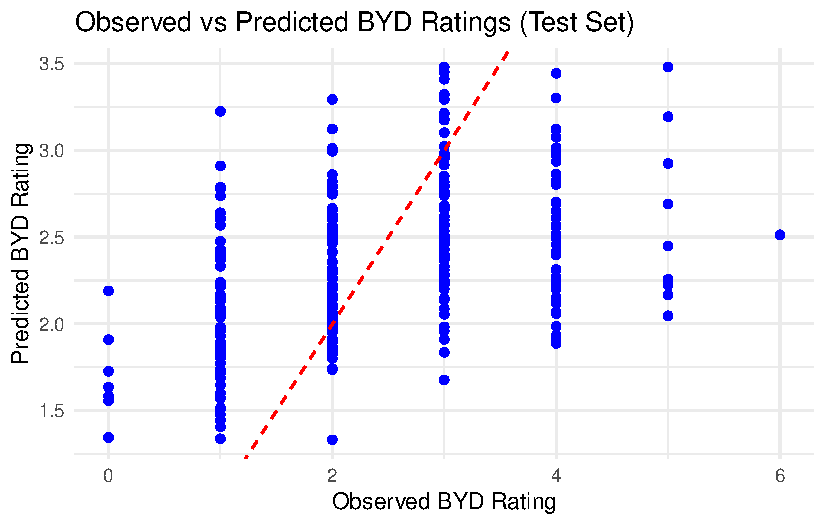
\includegraphics[keepaspectratio]{untitled_files/figure-pdf/unnamed-chunk-7-1.pdf}}




\end{document}
